
\begin{figure*}[ht!] 
	\centering
	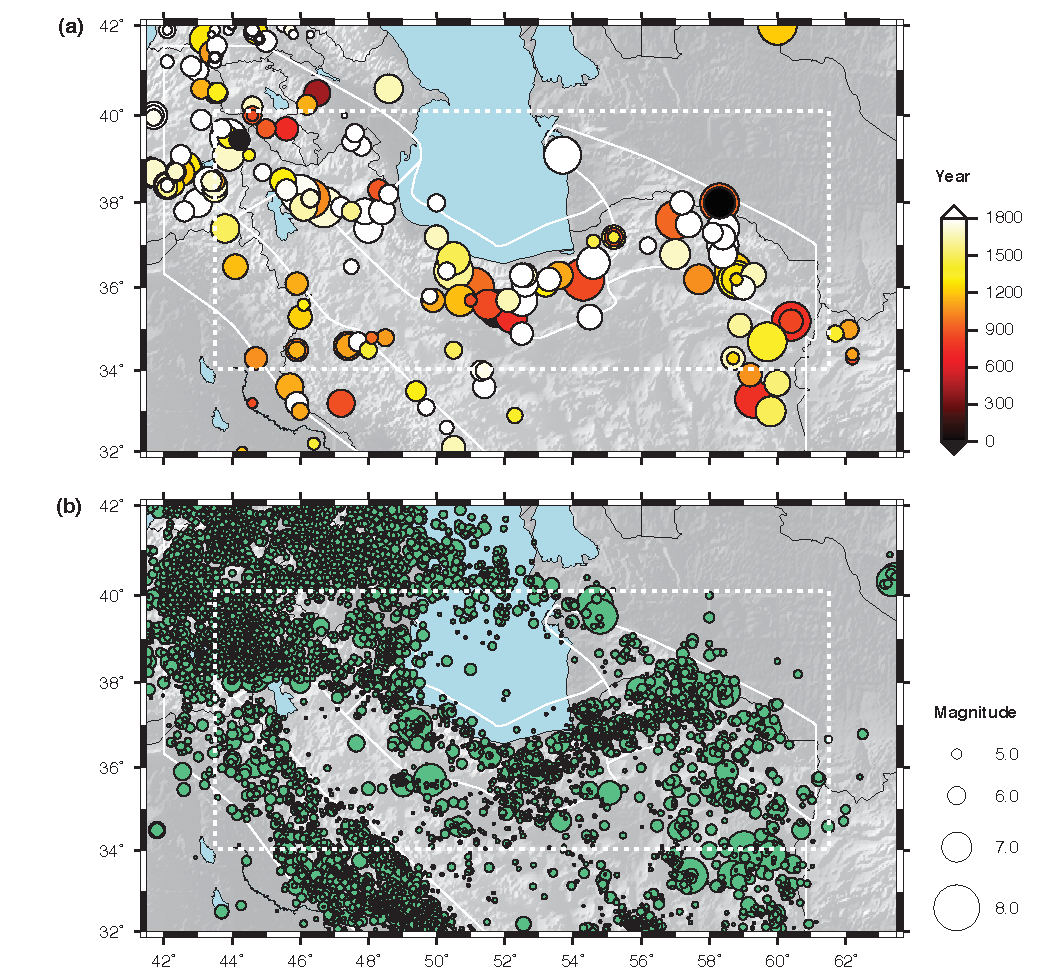
\includegraphics[width=0.9\textwidth]{figures/pdf/figure-03}
	\caption{Seismic catalog. (a) Historical seismicity prior to 1900. (b) Instrumental seismicity. Size of symbols is proportional to the magnitude of the events. In the case of the historical seismicity catalog, the color fill indicates the year of the event.}
	\label{fig:selected}
\end{figure*}

\section{Seismic Catalog}

A fundamental step in regional seismic hazard analysis is the compilation of a robust seismic catalog including reliable information about both historically documented and instrumentally registered earthquakes. Notable previous efforts to compose uniform earthquake catalogs for Iran include but are not limited to \citet{moinfar1994}, \citet{Berberian1994}, and \citet{Ambraseys2005}. These studies, however, often differ from each other in their use of magnitude scales or magnitude conversion rules and the extent to which they accept historical accounts as reliable data. According to \citet{Ambraseys2005}, for instance, there is scattered evidence of earthquakes as far back as the third millennium B.C. \citet{Mirzaei1997}, on the other hand, provides a comprehensive list of studies and collects earthquake information uniformly converted to surface wave magnitude, $M_s$, that date back to the 4th century B.C., and through 1994. While historical seismicity may be arguable, instrumental data is more easily available through agencies such as the International Institute of Earthquake Engineering and Seismology (IIEES); the Iranian Seismological Center (IRSC), at the University of Tehran; and the Building and Housing Research Center (BHRC), who operates Iran's Strong Motion Network see \citep[see additional details in][]{Karimiparidari2013}.



% Many most of attenuation relationship use  moment magnitude $M_w$ as an input for the equation \citep{Douglas2011}. Moment magnitude is not suffering from saturation and has physical meaning \citep{Kanamori1977}. Due to mentioned reasons Mw has become a most appropriate magnitude scale in recent studies. 

%  \citet{Karimiparidari2013}compiled a uniform earthquake catalog for Iran and adjacent areas, using international and national databanks until April 2010.  They developed relationships between moment magnitude and other magnitude based on orthogonal regression.  They removed the dependent events (aftershocks and foreshocks) using the procedure by \citet{Gardner1974}. The catalog of events with magnitude equal and above Mw 5.5 is provided. 
% \citet{Shahvar2013} presented a unified and homogeneous catalog for the Iranian plateau $(M_w >= 4)$, created by merging data from two local catalogs and seven international agencies for 1900-2011 period. They used orthogonal regression method \citep{Castellaro2006} to derive magnitude conversion relation. By removing foreshocks and aftershocks according to the procedure detailed in Uhrhammer(1986), they also provided declustered version of the catalog.

% The recent unified catalog for Middle East region is published as a part of Global Earth Model (GEM) and the Earthquake Model of the Middle East (EMME) project by \citet{Zare2014}. They used all historical (pre-1900), early and modern instrumental events up to 2006. The catalog contains data from Alborz-Azerbaijan, Afghanistan-Pakistan, Saudi Arabia, Caucasus, Central Iran, Kopeh-Dagh, Makran, Zagros, and part of Turkey. The magnitude of all events are converted to Mw through relationships which is derived at previous studies or newly derived at the study relationships. They declustered data through different methods including \citet{Gardner1974}, Uhrhammer(1986), \citet{Reasenberg1985}, and Gruenthal. \citet{Zare2014} provided the catalog completeness for different magnitude range using  the cumulative frequency-magnitude distribution of  \citet{Gutenberg1944} and \citet{richter1958}, and frequency magnitude distributaion of ZMAP \citep{Wiemer2001} software. The methods confirms the results of each other. 

% In this study we consider earthquakes with Mw equal and greater than 3. Earthquakes with magnitude 3 are not considered as a structural threat, however, the epicenter of earthquakes with magnitude $M_w 3$ are a  susceptible location for future bigger earthquakes.  According to our preliminary data processing based on IIEES data, Iranian catalog for earthquake with magnitude greater and equal 3, is complete from 2005. In order to make sure about the completeness of the catalog, we use IIEES data from 2000. We used the EMME project data provided by \citet{Zare2014} up to 2000. Fig.~\ref{fig:historical} represents the historical data (pre 1900) in the study region. 

% \subsubsection{Magnitude Conversion}

% The catalog of recorded earthquake from 2000-2015 which is downloaded from IIEES is reported the earthquake based on different magnitude scale. We converted the $M_L$, $M_s$, and $mb$ magnitudes through conversion relationships which is defined in \citet{Zare2014}. There also some of data which is recorded in $M_D$ (Duration magnitude). These data are reported by International Seismological Centre (ISC).  \citet{Deniz2010}, developed a set of empirical equations to convert earthquake magnitudes in $mb$, $M_D$, $M_L$ and $M_s$ scales to the $M_w$ scales using orthogonal regression procedure. They used data of earthquake that occurred in Turkey from different data centers including ISC. In this study we use the conversion equation of \citet{Deniz2010} to convert the Md to Mw. Although they defined the equation based on $M_w>=4.5$, we extrapolate the equation for lower magnitude. We believe having those earthquakes, even with small error  in magnitude is important for estimating an accurate "a" value  in Gutenberge-Richter equation.

% \begin{figure*}[!ht] 

% \centering
% \includegraphics[scale=0.4]{figures/pdf/Figure2.pdf} 
% \caption{Historical earthquakes of Iran (pre 1900). Different colors represent different year of occurrences and size of circles are proportional to the earthquake magnitude. }
% \label{fig:historical}
% \end{figure*}


% \subsubsection{Declustering}

% It is generally assumed that the seismicity of each tectonic seismic source follows a Poissonian occurrence process. Therefore, in order to accomplish this, we declustered the earthquake catalog. In compiling the catalog of events, foreshocks and aftershocks were removed using a declustering methodology \citep{Gardner1974}. For north Iran (lon: 42-62.5, lat: 33-41), from 7478 earthquake event we removed 605 Foreshocks and 2917 aftershocks.
% Whole data that we used for seismicity parameters of Zagros and Central Iran tectonic seismic regions are not included in these numbers. Fig.~\ref{fig:instrumental} shows the epicenter of declustered instrumental  earthquakes.


% \begin{figure*}[!ht] 

% \centering
% 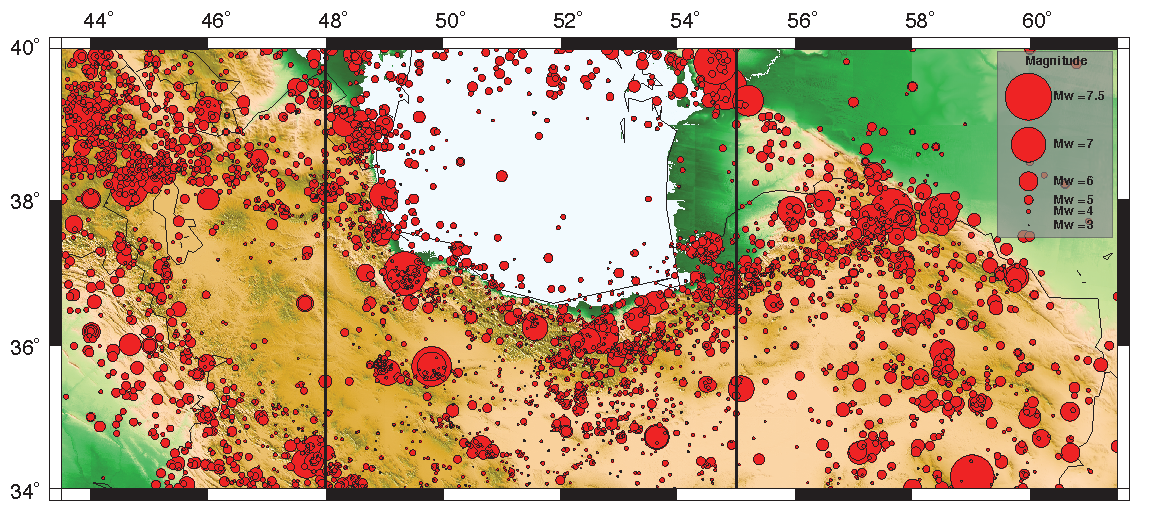
\includegraphics[scale=0.25]{figures/pdf/Figure3.pdf} 
% \caption{Declustered instrumental seismicity map (after 1900) of Northern Iran. The study areas are separated at longitude of 48$^{\circ}$ and 55$^{\circ}$ . } 
% \label{fig:instrumental}
% \end{figure*}


% \subsection{Divisions}

% As we discussed earlier (see the Introduction section), classifying the tectonic seismic regions has been a controversial debate. In this study we consider two seismic tectonic models. First model is according to \citet{Mirzaei1998} and \citet{Karimiparidari2013} classification, which includes Azerbaijan, Alborz, Kopek Dagh, and part of Central Iran, and Zagros, the second model is a uniform model for the whole north Iran.  


% *********************************************************************************************************************
% *********************************************************************************************************************

% Naeem's original Text
% ---------------------

% \subsection{Historical  and Instrumental Seismicity}

% Uniform earthquake catalog is the most important factor in seismic hazard analysis of a region.  Different studies have been conducted in order to prepare a uniform catalog for Iranian Earthquake. Historical event interpretation and different magnitude conversion relationships are some of the factors which make all these catalogs different. Among different sources \citet{Ambraseys2005}, \citet{Berberian1994}, and \citet{moinfar1994} are some of the main sources for Iranian earthquake catalog. These catalogs contain historical and instrumental earthquakes that have been reported in literature and national and international networks. According to \citet{Ambraseys2005}, there are some scattered indication of earthquake effects  back to third millinuim BC. However, adequate documentary coverage of individual events begins from seventh century A.D. \citet{Mirzaei1997} provided a comprehensive list of studies that have been done in compilation a uniform catalog for Iranian earthquakes in order to prepare a uniform catalog of earthquake (all earthquakes are converted to surface wave magnitude Ms) for seismic hazard assessment in Iran. The catalog is covering the period of 4th century B.C. through 1994. The instrumental data is achievable from three national agencies including IIEES, International Institute of Earthquake Engineering and Seismology; IRSC, The Iranian seismological center, University of Tehran; and BHRC, Building and Housing Research Center (Iran Strong Motion Network) (For more information about these networks see \citet{Karimiparidari2013}).


% Many most of attenuation relationship use  moment magnitude $M_w$ as an input for the equation \citep{Douglas2011}. Moment magnitude is not suffering from saturation and has physical meaning \citep{Kanamori1977}. Due to mentioned reasons Mw has become a most appropriate magnitude scale in recent studies. 

%  \citet{Karimiparidari2013}compiled a uniform earthquake catalog for Iran and adjacent areas, using international and national databanks until April 2010.  They developed relationships between moment magnitude and other magnitude based on orthogonal regression.  They removed the dependent events (aftershocks and foreshocks) using the procedure by \citet{Gardner1974}. The catalog of events with magnitude equal and above Mw 5.5 is provided. 
% \citet{Shahvar2013} presented a unified and homogeneous catalog for the Iranian plateau $(M_w >= 4)$, created by merging data from two local catalogs and seven international agencies for 1900-2011 period. They used orthogonal regression method \citep{Castellaro2006} to derive magnitude conversion relation. By removing foreshocks and aftershocks according to the procedure detailed in Uhrhammer(1986), they also provided declustered version of the catalog.

% The recent unified catalog for Middle East region is published as a part of Global Earth Model (GEM) and the Earthquake Model of the Middle East (EMME) project by \citet{Zare2014}. They used all historical (pre-1900), early and modern instrumental events up to 2006. The catalog contains data from Alborz-Azerbaijan, Afghanistan-Pakistan, Saudi Arabia, Caucasus, Central Iran, Kopeh-Dagh, Makran, Zagros, and part of Turkey. The magnitude of all events are converted to Mw through relationships which is derived at previous studies or newly derived at the study relationships. They declustered data through different methods including \citet{Gardner1974}, Uhrhammer(1986), \citet{Reasenberg1985}, and Gruenthal. \citet{Zare2014} provided the catalog completeness for different magnitude range using  the cumulative frequency-magnitude distribution of  \citet{Gutenberg1944} and \citet{richter1958}, and frequency magnitude distributaion of ZMAP \citep{Wiemer2001} software. The methods confirms the results of each other. 

% In this study we consider earthquakes with Mw equal and greater than 3. Earthquakes with magnitude 3 are not considered as a structural threat, however, the epicenter of earthquakes with magnitude $M_w 3$ are a  susceptible location for future bigger earthquakes.  According to our preliminary data processing based on IIEES data, Iranian catalog for earthquake with magnitude greater and equal 3, is complete from 2005. In order to make sure about the completeness of the catalog, we use IIEES data from 2000. We used the EMME project data provided by \citet{Zare2014} up to 2000. Fig.~\ref{fig:historical} represents the historical data (pre 1900) in the study region. 

% \subsubsection{Magnitude Conversion}

% The catalog of recorded earthquake from 2000-2015 which is downloaded from IIEES is reported the earthquake based on different magnitude scale. We converted the $M_L$, $M_s$, and $mb$ magnitudes through conversion relationships which is defined in \citet{Zare2014}. There also some of data which is recorded in $M_D$ (Duration magnitude). These data are reported by International Seismological Centre (ISC).  \citet{Deniz2010}, developed a set of empirical equations to convert earthquake magnitudes in $mb$, $M_D$, $M_L$ and $M_s$ scales to the $M_w$ scales using orthogonal regression procedure. They used data of earthquake that occurred in Turkey from different data centers including ISC. In this study we use the conversion equation of \citet{Deniz2010} to convert the Md to Mw. Although they defined the equation based on $M_w>=4.5$, we extrapolate the equation for lower magnitude. We believe having those earthquakes, even with small error  in magnitude is important for estimating an accurate "a" value  in Gutenberge-Richter equation.

% \begin{figure*}[!ht] 

% \centering
% \includegraphics[scale=0.4]{figures/pdf/Figure2.pdf} 
% \caption{Historical earthquakes of Iran (pre 1900). Different colors represent different year of occurrences and size of circles are proportional to the earthquake magnitude. }
% \label{fig:historical}
% \end{figure*}


% \subsubsection{Declustering}

% It is generally assumed that the seismicity of each tectonic seismic source follows a Poissonian occurrence process. Therefore, in order to accomplish this, we declustered the earthquake catalog. In compiling the catalog of events, foreshocks and aftershocks were removed using a declustering methodology \citep{Gardner1974}. For north Iran (lon: 42-62.5, lat: 33-41), from 7478 earthquake event we removed 605 Foreshocks and 2917 aftershocks.
% Whole data that we used for seismicity parameters of Zagros and Central Iran tectonic seismic regions are not included in these numbers. Fig.~\ref{fig:instrumental} shows the epicenter of declustered instrumental  earthquakes.


% \begin{figure*}[!ht] 

% \centering
% 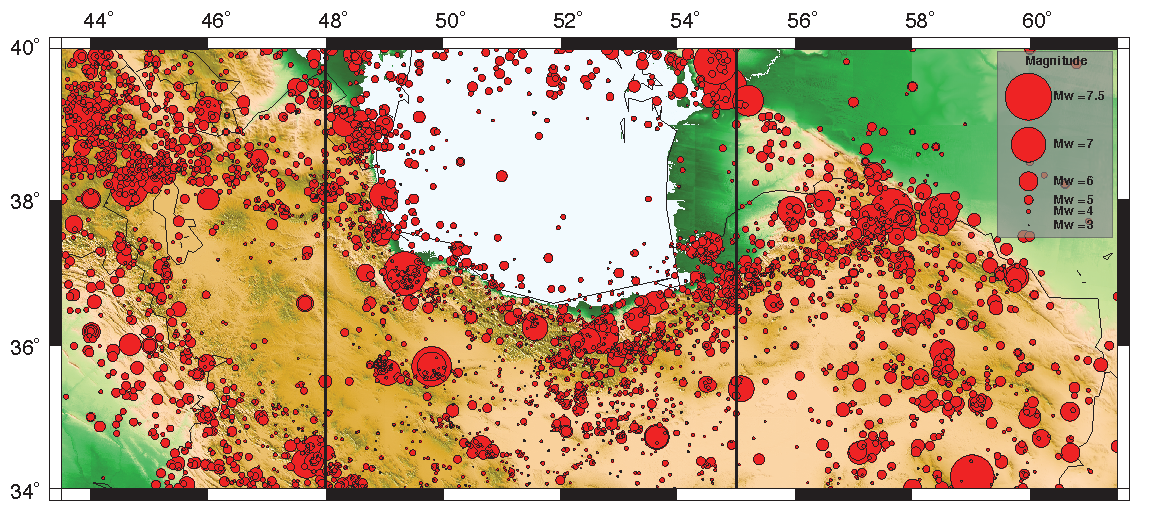
\includegraphics[scale=0.25]{figures/pdf/Figure3.pdf} 
% \caption{Declustered instrumental seismicity map (after 1900) of Northern Iran. The study areas are separated at longitude of 48$^{\circ}$ and 55$^{\circ}$ . } 
% \label{fig:instrumental}
% \end{figure*}


% \subsection{Divisions}

% As we discussed earlier (see the Introduction section), classifying the tectonic seismic regions has been a controversial debate. In this study we consider two seismic tectonic models. First model is according to \citet{Mirzaei1998} and \citet{Karimiparidari2013} classification, which includes Azerbaijan, Alborz, Kopek Dagh, and part of Central Iran, and Zagros, the second model is a uniform model for the whole north Iran.  
